%
% Documento: Disposições
%

\chapter{Implementação}

    Neste capítulo irei abordar as tecnologias de utilizadas para a codificação do framework,
    os modulos e suas classes expostas para o usuario e as ferramentas utilizadas para controle de versão
    e publicação do framework.


\section{Tecnologias Utilizadas}

    Para o desenvolvimento do framework foi utilizado apenas como linguagem para desenvolvimento o Python
    e para a manipulação e integração com o browser a biblioteca em python do Selenium Webdriver. Por ser um
    projeto que visa ser o mais simples e leve possivel apenas os modulos padrões do python estão sendo utilizado
    para o desenvolvimento desta ferramenta.


    \subsection{Python}

        A escolha do Python \cite{python} foi devida porque ele trata-se de uma linguagem de programação fácil de aprender e poderosa.
        Possuindo uma estruturas dados de alto nível e uma abordagem simples, mas eficaz, para a programação orientada
        a objetos. Contendo uma Sintaxe elegante e tipagem dinâmica, juntamente com uma interpretação natural, tornam
        a linguagem ideal para criação dos scripts do pybot.

    \subsection{Selenium WebDriver}
        Selenium Webdriver \cite{webdriver} é um framework utilizado para se comunicar e enviar comandos para os browser
        em conjunto com um controlador de cada browser especifico. Em comparação com seu antecessor, Selenium RC, o Selenium Webdriver
        não precisa de um server para enviar os comandos para o browser. Utilizando comando nativos do sistema operacional ao invés de
        comando javascript, usados pelo Selenium RC, deixam o Selenium Webdriver uma excelente ferramenta para integração com diversos
        browser.

    \subsection{Git e GitHub}
        Para o controle de versões e alterações do codigo fonte do framework e scripts de exemplo foi utilizado a ferramenta
        Git \cite{git} em conjunto com os servidores do Github \cite{github} para hospedagem e gerenciamento. Com eles foi possivel
        fazer alterações dos codigos fontes em qualquer computador e gerenciar os erros e melhorias do framework.


\section{Modulos}

    O framework consiste em alguns modulos basicos, cada um com suas devidas utilidades e funções.
    A separação dos modulos foi dada com base em suas caracteristicas e funcionalidades.

    \begin{figure}[H]
        \vspace*{0,3cm}
        \centering
        \caption{Diagrama de Componentes}
        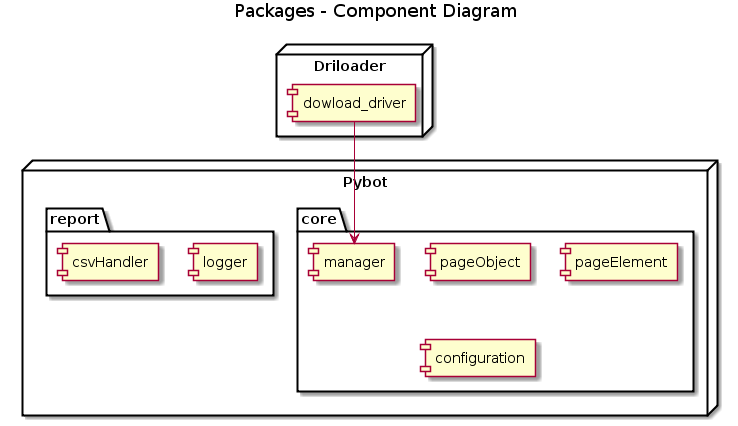
\includegraphics[width=1\textwidth]{./04-figuras/model}
        \label{fig:modules}
    \end{figure}

    \subsection{Core}
        \subsubsection{Manager}
        \subsubsection{Configuration}

    \subsection{Component}


        \subsubsection{WebElement}
        \subsubsection{PageObject}
        \subsubsection{PageElement}

    \subsection{Report}

        Estes modulo está destinado para geração de logs de execuções internas do framework, criação e controle
        de logs definidos pelos usuario e a criação de planilhas análiticas de dados extraidos das paginas.

        \subsubsection{Logger}
        \subsubsection{CsvHandler}
